\documentclass[]{final_report}
\usepackage{graphicx}
\usepackage{hyperref}
\usepackage[final]{pdfpages}
\usepackage{natbib}
\usepackage{booktabs}
\usepackage{multirow}
\usepackage{framed}
\usepackage{caption}
\usepackage{tikz}
\usetikzlibrary{timeline}
\usepackage{dirtree}

%%%%%%%%%%%%%%%%%%%%%%
%%% Input project details
\def\studentname{James King}
\def\reportyear{2018}
\def\projecttitle{Cooperative Strategies in Multi-Agent Systems}
\def\supervisorname{Kostas Stathis}
\def\degree{BSc (Hons) in Computer Science}
\def\fullOrHalfUnit{Full Unit} % indicate if you are doing the project as a Full Unit or Half Unit
\def\finalOrInterim{Interim Report} % indicate if this document is your Final Report or Interim Report

\begin{document}
	
\maketitle

%%%%%%%%%%%%%%%%%%%%%%
%%% Declaration

\chapter*{Declaration}

This report has been prepared on the basis of my own work. Where other published and unpublished source materials have been used, these have been acknowledged.

\vskip3em

Word Count: 

\vskip3em

Student Name: \studentname

\vskip3em

Date of Submission: 

\vskip3em

Signature:

\newpage

%%%%%%%%%%%%%%%%%%%%%%
%%% Table of Contents
\tableofcontents\pdfbookmark[0]{Table of Contents}{toc}\newpage

%%%%%%%%%%%%%%%%%%%%%%
%%% Your Abstract here

\begin{abstract}

\end{abstract}
\newpage

\chapter{Aims, Objectives and Literary Survey}
Note: Documentation of the structure of my submission directory is in the appendix in chapter~\ref{appendix}, and description of where to find each report and program can be found in the summary of completed work in chapter~\ref{chapter:summary}.
\section{The Problem}
\label{section:problem}
To understand the aims and objectives of this project we must first grasp the history of the study of interaction between biological and computational agents (often known as intelligent agents in the field of computer science). It is important to distinguish between biological and computational agents as the study of natural selection and the evolution of cooperation in biological agents has a long and separate history from the study of intelligent agents in computer science.\\
The background to my project is covered in my first two reports (included in the appendix in chapter~\ref{appendix}). I will be applying this knowledge in a more convenient format for the interim report here, my two reports provide a more in depth study on the topic of the evolution of cooperation and indirect reciprocity.\\
As explained in my first report (on the evolution of cooperation in relation to game-theory and different game-theoretic mechanisms to aid it), early Darwinian evolutionary theory was groundbreaking, however both opponents and even proponents of evolution such as Peter Kropotkin~\cite{kropotkin1902mutual} (a Russian evolutionary scientist and political activist) found it fell short in explaining cooperative phenomena.\\
Cooperation is the idea of helping others at a detriment or cost to yourself. Of course, this concept is a key part of the natural world. For example, the act of parents supporting their children and vice-versa in human family groups. There are even interspecies examples such as that of the Meerkat and Drongo Bird~\cite{bbcafrica}.\\
The problematic question posed by the phenomena of cooperation is the idea from the theory evolution: the survival of the fittest~\cite{spencer1864principles}. This idea pushes individuals to compete for resources, so why does cooperation exist when there is a process actively pushing for competition? How did cooperation evolve in a world focused on competition?

\section{Cooperation Aids}
There have been a number of attempts to explain the phenomena of cooperation~\cite{kropotkin1902mutual, selfish_gene, evolution_of_cooperation, five_rules_coop}. In his book `The Selfish Gene'~\cite{selfish_gene} Richard Dawkins attempted to explain the idea that the real replicator in natural selection is the gene itself, which is self-interested in replication. As such, individuals are driven to working towards replication of the gene, not to improving our own personal fitness.\\
The idea of being driven towards the replication of our genes comes under the banner of Kinship Theory, highlighted by Axelrod and Hamilton in their paper~\cite{evolution_of_cooperation} as one of the theories seeking to explain cooperation. Hamilton wrote a paper on Kinship Theory earlier in his academic career~\cite{kinhamilton}, explaining his version in which agents are encouraged to cooperate as they are interested in improving `inclusive fitness' over their own individual fitness. Inclusive fitness refers to the fitness of both themselves and their relatives; the closer the relative the more they have an effect on an agent's inclusive fitness.\\
The main mechanism highlighted by Axelrod and Hamilton~\cite{evolution_of_cooperation} is, in popular culture, known as the game `the iterated prisoner's dilemma'. The iterated prisoner's dilemma uses the idea of direct reciprocity to aid in the evolution of cooperation. This idea being: if I scratch your back, you'll scratch  mine. In a round of the prisoner's dilemma, both agents simultaneously choose whether to cooperate or defect. A single prisoner's dilemma round provides no aid, but if the rounds are repeated, agents are encouraged to cooperate if historically there has been cooperation from the other agent with whom they're interacting. Another reason to cooperate is the payoff matrix given in table~\ref{tab:ipdpayoffmatrix}. Multiple rounds of both agents cooperating gives both higher social welfare (overall points accrued~\cite{kostas_deductive}) and greater individual payoff than multiple rounds of mutual defection.
\begin{framed}
	\begin{center}
		\begin{tabular}{c|c|c}
		\multirow{2}{*}{Player A} & \multicolumn{2}{c}{Player B}\\		
		& Cooperation & Defection\\
		\hline
		\multirow{2}{*}{Cooperation} & A=3 & A=0\\
		& B=3 & B=5\\
		\hline
		\multirow{2}{*}{Defection} & A=5 & A=1\\
		& B=0 & A=1\\
		\end{tabular}
		\captionof{table}{The payoff matrix in a typical iterated prisoner's dilemma game (such as Axelrod and Hamilton's). A=x, B=y where x denotes the payoff for A and y the payoff for B.}
		\label{tab:ipdpayoffmatrix}
	\end{center}	
\end{framed}
Direct reciprocity and Kinship Theory (or kin selection) are two of the five rules presented in Martin A. Nowak's paper `Five Rules for the Evolution of Cooperation'~\cite{five_rules_coop}. The other three rules use different versions of reciprocity mechanisms. Network reciprocity is similar to the iterated prisoner's dilemma. Axelrod and Hamilton's approach~\cite{evolution_of_cooperation} uses a round-robin tournament where all players interact with every other player. Network reciprocity is set aside from this style of direct reciprocity as it is played on a graph with players as the nodes, and the edges denoting who interacts with whom.\\
Another of the five rules, group selection, builds upon direct reciprocity. In group selection a population is separated out into smaller subpopulations. The players in these subpopulations only interact and reproduce within their subpopulation group. The group sizes fluctuate based on how fast agents reproduce inside them (dependent on the agents' fitness scores). If a group gets to a certain size, it has a chance of splitting, and when one group splits another group is removed. The effect of this is selection on two levels: individually and between groups, aiding the evolution of cooperation.\\
The last mechanism presented by Nowak and the one I am most interested in, is indirect reciprocity. The idea behind this mechanism is slightly less intuitive than direct reciprocity: if I scratch your back, hopefully later on someone else will remember and scratch my back. Actions in indirect reciprocity are different to direct reciprocity as they do not involve both agents acting. Only the donor of the donor-recipient interaction pair can choose to cooperate or defect, the payoffs of which are presented in table~\ref{tab:indirectpayoffmatrix}.
The indirect reciprocity mechanism utilizes the idea of reputation. Cooperative acts may result in bettering the donor's reputation whereas defecting may result in a loss of reputation. How agents view the reputation of another, depends upon their implementation. Two important implementations described in my second report are the standing strategy~\cite{leimarhammer} and using image scores~\cite{evol_indirect_image}. Agents have the opportunity to base their decisions on these reputations. Sommerfeld \textit{et al.}~\cite{gossip_alt} put forward that the social action of gossip can help agents spread information in regards to agents reputations.
\begin{framed}
	\begin{center}
		\begin{tabular}{c|c|c}
		\multirow{2}{*}{Donor Action} & \multicolumn{2}{c}{Payoffs}\\		
		& Donor & Recipient\\
		\hline
		Cooperation & -1 & 2\\
		\hline
		Defection & 0 & 0\\
		\end{tabular}
		\captionof{table}{The common payoff for most indirect reciprocity models}
		\label{tab:indirectpayoffmatrix}
	\end{center}	
\end{framed}

\section{Theory Surrounding Intelligent Agents and Multi-Agent Systems}
In my third report in the appendix chapter~\ref{appendix} I have covered the theory surrounding intelligent agents and multi-agent systems. Agents, as described by Russell and Norvig~\cite{russell2016artificial}, are anything that perceives and acts upon its environment. Agents can be built using a number of architectures, some of which are seemingly more intelligent than others. Russell and Norvig highlight 5 such architectures ranging from agents which simply act in reflex to their environment to agents that actively learn from their percepts.\\
The idea that an agent is anything the perceives and acts upon it's environment could be considered a `weak' notion of agency, even in comparison to Wooldridge and Jennings' `weak' notion of agency~\cite{wooldridge_jennings_1995}. Their paper stipulates that agents must be able to exhibit these 4 properties: autonomy, social ability, reactivity and proactivity.\\
Autonomy is considered to be operating without direct human or other agent intervention, with the agent having control over their internal state and actions. Social ability is defined as the ability of agents to interact with other agents (possibly biological) using an agent communication language. Reactivity is the ability to perceive their environment and act upon the changes in it. Proactivity makes Wooldridge and Jennings'~\cite{wooldridge_jennings_1995} notion stronger than Russell and Norvig's~\cite{russell2016artificial} as it stipulates agents must not simply be reactive to their environment but are also able to exhibit goal-directed behaviour.\\
To be able to satisfy the properties laid out by Wooldridge and Jennings~\cite{wooldridge_jennings_1995} and the definition of an agent from Russell and Norvig~\cite{russell2016artificial} agents need an environment to reside in. The possible environments are endless. An agent is built to work in a specific environment, the reason for an agents existence varies but often agents will attempt to complete specific tasks delegated to them.\\
Multi-agent systems are systems consisting of a combination of an environment and a number of agents perceiving and acting within it. Interactions can generally occur between both the environment and other agents in the system.


\section{Relevance of The Problem and Indirect Reciprocity to Multi-Agent Systems}
The societies which are simulated in the theories and experiments presented by Axelrod, Hamilton and Nowak~\cite{evolution_of_cooperation, five_rules_coop} are strikingly similar to multi-agent systems. The models include groups of players residing in an environment interacting with each other, leading naturally to using these game-theoretic approaches to modelling interactions in multi-agent systems.\\
As agents act autonomously in a multi-agent system, why should one agent cooperate with another at a cost to themselves? From a developer's viewpoint, they can see the possibilities that if agents work together agents can accomplish so many brilliant things. From the agent's viewpoint though, why should that agent trust that if they cooperate, their good actions will not be taken advantage of?\\
This is the problem in section~\ref{section:problem} reformulated for multi-agent systems. From a developer's perspective working on these sorts of systems, their goal is to encourage cooperation between agents but also not leave their agents or system of agents open to abuse. How can developers achieve this goal?\\
One way to approach this problem is to study how other environments have achieved this. One such environment that has achieved the evolution of cooperation, that we have identified earlier in this report, is the environment we live in, nature itself. Though nature encourages competition it has also led to cooperation between biological agents. So how can we learn from the processes nature employs?\\
We can apply the processes identified by game-theory and Kinship Theory to model multi-agent systems by implementing multi-agent systems that run these processes. Using a similar mechanism to indirect reciprocity Mui \textit{et al.}~\cite{Mui:2002:NRM:544741.544807} explored the role of reputation in the evolution of cooperation in multi-agent systems. The paper uses a number of different notions for reputation, one similar to Nowak's observer-based reputation, where an agent changes their view of another agent depending on the actions it views of the other agent. Their experiments found a large number of interactions were needed per generation for cooperative agents to dominate.\\
The mechanism/process I have chosen and outlined in my report on indirect reciprocity was chosen as I believe it applies well to multi-agent systems for a number of reasons. Firstly agents who interact across large networks such as the internet may never interact again, so it is imperative to have a strategy for deciding on how to act in these singular interactions. My models use of indirect reciprocity and reputation will allow us to study specifically these sort of `sparse' interactions and the effectiveness of strategies in these interactions.\\
Another reason I believe my model matches multi-agent systems well is the social ability that it comes with. Nowak and Sigmund highlighted the importance of knowing another agents reputation to the success of the evolution of cooperation in an indirect reciprocity system~\cite{evol_indirect_image}. They found that the probability of knowing another agents reputation had to be greater than the cost to benefit ratio of the action for cooperation to evolve.\\
In my system, agents who know each other will be able share information via gossip on other agents. The shared information increases the chances of knowing a certain agents reputation and in turn, helps defend against generally cooperative or `nice' agents from being exploited. However, it also leads to another avenue of attack through spreading misinformation. This mechanism of information sharing could be used as a defence against exploitation, but it is important to understand how best to implement it and how effective it is before such an option is chosen.\\
One of the four properties laid out by Wooldridge and Jennings~\cite{wooldridge_jennings_1995} is autonomy, which includes control over the agent's own internal state. The fact that in my model reputation is not a centrally managed concept but is part of the internal state, brings the system closer to a truly decentralised multi-agent system architecture.\\
Though reproduction itself doesn't, in fact, occur in multi-agent systems, it is likely that agent systems will be replaced and upgraded. The replacing systems will probably follow strategies that are known as effective by the developers. My reproduction mechanism aims to show how this replacement will take place, by assigning more likelihood for reproduction of an agent to occur if the strategy is successful. The reproduction may tend towards a defecting agent if they are more successful and vice-versa.\\
For further information on my model please refer to my second report on indirect reciprocity, strategies for agents and the development of a concrete model to implement in the appendix in chapter~\ref{appendix}.

\section{Project Specification, Aims and Objectives}
From the sections above we can recognise that the study of indirect reciprocity and other mechanisms is important for the development of multi-agent systems and the prevention of exploitation by malicious agents. My project aim is to work on studying the model of indirect reciprocity I have defined and it's effectiveness in aiding the evolution of cooperation.\\
I will be doing this by implementing the model as a multi-agent system with a variety of strategies including the image scoring discriminator and standing strategy described in my second report. The specification for my system design has been described in my third report. Further to the multi-agent system, I will be implementing a web application to run the environment. The web application will allow a user to select agents for their simulation and then run the simulation. The web application aims to act as an educational system on direct and indirect reciprocity (direct reciprocity has already been implemented using a preexisting library as a proof of concept for the web application).\\
After the simulation has ended a user will be redirected to an analysis of the simulation, where they will be able to examine the success of the model and strategies in regards to the evolution of cooperation. Analysis data will be held in a database for reuse later on. I will be using this system myself to examine the model and strategies effectiveness, alongside how the setting of parameters such as the number of interactions per generation are required for cooperation to evolve - as was examined by Mui \textit{et al.}~\cite{Mui:2002:NRM:544741.544807}.\\\\
To sum up my aims:
\begin{itemize}
	\item Implement the mechanism I have outlined in a multi-agent system
	\item Implement a number of strategies for use in the model
	\item Examine the relevance and success of the mechanism I have outlined in regards to the evolution of cooperation in multi-agent systems
	\item Examine the success of different strategies and trust models for agents in the system
	\item Explore how social ability/gossip can affect the evolution of cooperation in a multi-agent system
	\item Explore the various parameters that are important in the system in regards to what setting is required for cooperation to evolve
\end{itemize}

\chapter{Planning and Timescale}
\label{chapter:planningtime}
In my project plan (which can be found in my appendix in chapter~\ref{appendix}) I decided on using 2-week sprints to manage the time at which milestones should be met. In sprint 1, I was to reach 3 milestones: 2 proof of concept applications and a report on the evolution of cooperation.\\
Having done a lot of research over the summer on the evolution of cooperation and a tutorial for Flask I believed these reachable targets. Unfortunately, I overestimated how much I could do. As it can be seen in my diary in chapter~\ref{chapter:Diary} I did not complete this work in the first two weeks.\\
This was, unfortunately, a recurring theme; milestones were often not met. I feel that I underestimated the duration needed to reach milestones for 4 reasons. The first is that I work hard to make what I do the best standard I can, meaning I will often add time to a task to perfect it, which sets me back. Another is that I did not leave enough time for prototyping and designing my programs. The third is that I did not plan my tasks in enough detail, I simply attempted to hit a deadline each time. Lastly, I underestimated the amount of work other modules would require of me and the coursework I would need to complete for these.\\
This is not to say that I am completely off balance in the project. I have the milestones for term 1 completed, even if they were late. I have even implemented the gossip and onlooker features from the first two milestones of the second term. The issue with the implementation that I have completed so far is that it was often not completed in time for the milestone and as such, I ended up rushing some of the work. This led to a lack of extensive documentation and testing, and also a lack of detailed design work.\\
I am going to do two things to mitigate the issues I have had in this term in second term. One of which is to use the Christmas period to ensure documentation and testing is up to scratch before I begin any second term work.\\
Moving into the second term, I will also address these issues by creating a stricter plan. This includes more carefully planning design and prototyping time, and the processes required around implementation such as documentation and testing. Now I am versed more thoroughly in the project, I am in a better position to split milestones into far more fine-grained tasks. I shall again be organising my work in sprints but will be more strict on when these fine-grained tasks should be completed rather than having high-level milestones to work towards. Fine-grained tasks suit the scrum methodology more than high-level milestones, so I hope to be more successful using this.


\chapter{Summary of Completed Work}
\label{chapter:summary}
\section{Proof of Concept}
\subsection{Proof Of Concepts}
After finishing my project plan I embarked on the implementation of two proof of concept programs. Both involved learning technologies that are new to me. The first proof of concept I had already begun work on in the summer was implementing a web application to select agents and parameters to run matches and tournaments of direct reciprocity using the Axelrod-Python library to run the matches and tournaments in the back-end.\\
For this web app, I used Python and learnt the Flask microframework to develop the server-side alongside the SQLAlchemy ORM and SQLite for development. To learn the Flask microframework and its ecosystem I had taken the course `The New and Improved Flask Mega Tutorial'~\cite{flask_tut} in preparation over the summer. This greatly improved my web development knowledge and skills, but I found I needed more knowledge for developing the front-end to select a dynamic number of agents. As such I took a crash course in React.js~\cite{react_crash_course}. React has a number of features that Flask's template engine Jinja2 just can't accomplish. In my work I used the PyCharm IPSE and its various tools, such as the Flask framework support tools.\\
Using the skills I accrued from these two courses and my knowledge of direct reciprocity, the Axelrod-Python library and Python itself, I successfully developed the web application. This application uses a wide array of technologies such as Redis, Bootstrap and others previously mentioned. I feel that it really helped develop my skills in web development, which will be beneficial to my development of a nice graphical user interface for running and analysis of tournaments and also the educational aspects of my final product. To run the web application see my notes in the README.md file in the top-level of my submitted directories.\\
My second proof of concept application was a small web service written in Prolog. Again the technologies used for this were new to me so I followed a tutorial `Creating Web Applications in SWI-Prolog'~\cite{swi_web_tut} and continuously consulted the SWI-Prolog documentation. The purpose of this proof of concept application was to practice and demonstrate that I can create web services using Prolog before I went ahead and developed the agents service.\\
This second proof of concept was successful and I proved to myself that I could create an adequate web service. The outcomes of this were a knowledge that I immediately put to use in creating the agents service and also a guide on how I can do this using the JSON format and certain methods of error handling among other things.

\section{Practical}
Moving on from the proof of concept programs I started on design and implementation of the multi-agent system including the agents service and environment.
\subsection{Agents Service and API}
For SWI-Prolog there is a lack of an integrated project support environment or even an integrated development environment (except for in GNU EMACS which I do not have experience with). The tooling I have been using for the development of the agents service is the syntax highlighter in sublime text, and for testing the experiment bed (provided as part of the multi-valued fluent cached event calculus) and the Prolog unit-test framework. I have used this to test belief revision in the file tests.pl under the directory AgentsService/src/mvfcec/src. To run this compile the tests.pl in SWI-Prolog (tested on v7.6.4) and run the predicate run\_tests(percepts).\\
Further unit testing and documentation of the system is required to improve coverage and understandability of the code. However, testing of the functionality of the system using API testing has been extensive, the API testing code can be found in the directory NatureEngineWebApp/tests/agents\_service\_testing. I decided to write my own testing using the python requests library and unittest framework instead of a tool such as Postman as I can easily commit the tests using git without needing to pay and the python requests library and unittest framework are both extremely easy and nice to use. I have also used these previously so they required no extra learning.\\
The API has been documented using the RESTful API Markup Language RAML (based on YAML). RAML has tooling surrounding it to easily convert a .raml file into a user understandable format, such as the raml2html tool that I have used to generate the file main.html under the directory AgentsService/api\_docs.\\
The API is designed to use the correct HTTP methods, uniform resource indicators to access and manipulate resources and to generally conform to RESTful API principles outlined at \url{https://restfulapi.net/}.\\
The agents service code for the web service side of the program has been based on my learning from the proof of concept Prolog service. The code that runs the multi-valued fluent cached event calculus (mvfcec) has come from my supervisor Kostas Stathis. I have built on top of mvfcec with initiates\_at/3 predicates to define how an agent revises its beliefs using mvfcec (this is in the AgentsService/src/revise.pl file). Revision of beliefs has been implemented for when an agent is in an interaction, and when a standing strategy agent (both trusting and distrusting variants) receives gossip and interaction observation percepts.\\
A whole vertical slice has been implemented for defector, cooperator and standing strategy strategies. This means that they can receive percepts (refer to AgentsService/src/percepts.pl file), revise their beliefs and decide on actions at specific timepoints based on their knowledge at that point (refer to AgentsService/src/actions.pl).\\
The agents are built in the deductive reasoning style and using the concepts of beliefs, commitments, capabilities and logical theories as described in my system design report.\\
Further to this vertical slice it is also possible to query agents beliefs on when they were a donor, recipient, when two believe they were both in an interaction together and, if the agent is using the standing strategy, what they believe about the standing of another agent.\\
All this slice would be useless if users of the service were unable to find what strategies are implemented in the system. Users are able to retrieve the strategies from the /strategies URI as described in the main.html file. The implementation can be found in AgentsService/src/strategies.pl. The slice would also be useless if the service were unable to manage agent creation and assigning of strategies to them, this has been implemented in the agents.pl and communities.pl file. An agent is assigned to a community and generation, and also associated with a player id and strategy when created.

\subsection{The Environment}
The environment has been slightly tricky to implement because of the nature of the cycle step: send percepts to agents, get decisions from the agents and then execute these decisions (producing percepts). The cycle step easily introduces cyclic dependencies, high coupling and low cohesion in object oriented design.\\
I have been using umlet to design a class structure and execution sequence for the environment. Other tools in the development I have been using include the tools available in the Pycharm IPSE (linting, syntax highlighting, refactoring, built-in terminal, git support and unittest framework support), reStructuredText docstrings and sphinx for documentation, and the python venv which I had already set up for the web application.\\
For implementation I have the logic to select a number of strategies and simulate a community. The community simluation creates a first generation and after a number of cycles steps reproduces into the next generation, repeating the reproduction into a new generation a specified number of times. Each generation is simulated by running, for a set number of cycles, the steps: perceive, decide and execute. The perceive step handles sending percepts to the agents (including the percepts generated from the last cycle step's actions and the donor-recipient pair for this step). The decide step then asks the agents for their commitment to an action at the given timepoint. After decision making, the execute step, if necessary, alters player fitness and generates percepts for the next cycle. The environment also creates communities, generations and players correctly in the agents service.\\
Though the environment was written using a TDD approach, I recognise that the test coverage is not enough and feel that there are likely to be a few latent bugs. I will be writing more testing for this soon, in order to reveal these bugs using a smoke testing strategy. \\
Furthermore I will be working on increasing cohesion in the class structure as currently the generation class is large and responsibilities could be separated out. I will also be creating a class above the community class in the hierarchy, that calls the simulate method on the community object and then uses visitors or other analysis classes to produce results and analysis on the simulation.

\subsection{Tools, Techniques and Processes}
All my work is in a git repository hosted on GitHub. I have been using git by creating branches for specific tasks, such as API testing, API documentation etc. and then merging back into the master when complete.\\

\section{Theory}
I have completed 3 reports with the first focusing on the problem at hand as described in section~\ref{section:problem}, the second focusing on a specific solution to this problem, and the third on designing a system to simulate the model outlined in the second.

\subsection{Evolution of Cooperation Report}
\label{sub:evolcoop}
This report focuses on the problem at hand and the various theories and approaches taken to explain the evolution of cooperation. For the report, I reviewed past work surrounding the evolution of cooperation and theories to explain it. This review guided my development of a concrete model as delineated in my second report and served as a basis to extend my knowledge of the problem.\\
The report can be found in the directory ProjectReports/EvolCoop under the name EvolCoopReport.pdf.

\subsection{Indirect Reciprocity Report}
\label{sub:indirrec}
This report focused on examining the mechanism of indirect reciprocity in regards to being a mechanism aiding in the evolution of cooperation, its application to multi-agent systems and setting out a concrete model to implement.\\
I reviewed past work on indirect reciprocity and compared the various work. From this knowledge, I then specified the model I wished to implement and a few strategies I should implement and how should they be implemented.\\
The report can be found in the directory ProjectReports/IndirRec under the name IndirRec.pdf.

\subsection{System Design Report}
\label{sub:sysdesign}
So far in my reports and background work, I had mostly focused on the problem and game-theoretic aspects of the project. This report was different and focused on the design of my multi-agent system using the model I had set out in the second report.\\
I worked towards matching an architecture and design of the system and agents to the model and strategies I had set out previously. This report was influenced by my background reading in the domain of intelligent agents and multi-agent systems, but also the background work on indirect reciprocity I have completed and the implementation I already had.\\
Due to my findings in the report, I made some revisions to my design decisions and implementation, causing me (alongside other reasons) to redesign the environment.\\
The report can be found in the directory ProjectReports/SysDesign under the name SysDesign.pdf.

%%%% ADD YOUR BIBLIOGRAPHY HERE
\newpage
\bibliography{../../refs.bib}{}
\bibliographystyle{plain}
\addcontentsline{toc}{chapter}{Bibliography}
\footnote{A lot of my background theory work has been completed in my earlier reports so many of the references appear in those reports (see appendix)}
\label{endpage}

\chapter{Diary}
\label{chapter:Diary}
\subsection*{3:30 pm on September 28, 2018}
A catchup of the happenings so far.\\
Early steps and planning:\\
Towards the end of term project details were released. I began my research into the topic by watching youtube videos (https://www.youtube.com/watch?v=BOvAbjfJ0x0) on the iterated prisoner’s dilemma, reading the evolution of cooperation by Robert Axelrod and William D. Hamilton, and playing the evolution of trust game online (https://ncase.me/trust/).\\
The discussions with Kostas were helpful in augmenting this research. These meetings helped me decide that Python was the best option to implement the project in and introduced me to the concepts of gossip and communities – which I would not pin down until much later in the summer.\\
Research over the summer:\\
In the summer I researched into the topic of the iterated prisoner’s dilemma more and also how I should be using Python to implement this. I settled on using the Flask framework to create a web app to run these games, taking the Miguel Grinberg course Flask Mega-Tutorial to learn this. It was not until later that I would realise that using Flask would hamper my ability to interface between Python and Prolog to run the event (though I may still be able to use Prolog to implement strategies).\\ 
I continued with the idea that I would implement games, tournaments and a what I had believed to be a new idea called communities for this web application. For this I began development of the front-end and database of my web application that I dubbed The Nature Engine.\\
PyCon UK 2018 and a change of tack:\\
As a result of my research into python I decided to attend PyCon UK 2018 to expand my skills in it. At this conference, I joined in many workshops and listened to many talks on various parts of the python ecosystem. However the keynote speech on Monday was extremely interesting, the speaker is studying a PhD game theory at Cardiff University and spoke about the iterated prisoner’s dilemma and it impacts. It turns out that two other experts in the field were in attendance as well, all of which were core contributors to a library named Axelrod-Python. This library runs games, tournaments and much more.\\
With the realisation that most of my plan has already been implemented in a well tested mature library, I decided a change of tack was needed. One idea that the speaker had given me – in answer to a question about whether there were models for community-level interaction – was spatial tournaments. She had studied them for her MSc and wanted to point me in the right direction. This got me thinking that there are surely other models in game theory very closely related to this. \\
Post-PyCon research and the reformulation of my project:\\
It turns out these models do exist – which I discovered in the paper Five rules for the evolution of cooperation by Martin A. Nowak – and do not seem to be implemented in code at this current moment. There is still quite a decent amount of research about them. One that took my eye, which seemed to be very similar to what I had thought to be a new development of communities, known as group selection. This led to down to a reformulation of my ideas for The Nature Engine. To explore these alternative mechanisms noted in the five rules for the evolution of cooperation.\\
Return to university and meeting with Kostas:\\
With the past happenings in mind, I had a rough plan. I then had a meeting with Kostas to discuss my ideas with him. We talked at length about the different mechanisms and it soon became clear that I focused my project heavily on the game theory aspect of it and had moved away from the intelligent agents’ aspect. With this in mind, we bounced ideas around about how to integrate my ideas within an intelligent agents project. We decided to explore a very interesting idea to both me and Kostas that involved creating a Prolog service to run the decision-making component of the agents. This would involve slimming down parts of the project to keep the scope small enough for the time I had. My interest in the onlookers and gossip aspect of indirect reciprocity and completely separate strategies to direct reciprocity lead me to focus on indirect reciprocity.

\subsection*{10:57 am on October 4, 2018}
For this week of work, I have been focusing on finalising a solid project plan. Fleshing out the details of milestones, communicating my motivation for the project properly and exploring various mitigations I can take for foreseen risks. I feel as if I have got a bit bogged down with perfecting this (though I have begun a couple of pieces of proof of concept work) and I am now happy to have submitted.\\
This will now allow me to push on with the proof of concept work for the Prolog service and Flask web application, and also allow me to move onto my first report. I have a lot prepared for all 3 of these tasks and am ready to really get stuck into them, if I manage to get these finished early I may even be able to move onto the 2 more difficult reports.

\subsection*{9:43 am on October 12, 2018}
My two proof of concept apps are coming along nicely. For the Flask web app proof of concept, I now have a front-end working with its Axelrod-Python match library counterpart in the server, and I have designed and implemented a database structure to record the outcome of games. I have also created unit tests for the functions that convert from the representation in the Axelrod-Python library for game results and stats to the database model I have created and then to a representation suitable for displaying on my front end.\\
For the Prolog web service proof of concept, I have worked out the handling of URI endpoints, HTTP errors, HTML in Prolog (which is super weird and I won’t use it), sessions, running the server, building responses to requests, POST and GET methods, links and a few other bits. I am currently building them up using HTML to get data and display the results before I can use XML or JSON as these come later in the tutorial that I am using.\\
I am optimistic that working with a Prolog web service and Flask web app will work for my project quite nicely, but am concerned that I may be already getting behind as I said there is a report that I would hope to finish this week but simply haven’t had time. Luckily this report is linked to the next one I will be doing so I will do the reading for both at the same time and write at the same time, as I still need to finish the proof of concept web app. 

\subsection*{5:16 pm on October 19, 2018}
I have been adding to my Flask web application proof of concept application, I have taken tutorials on using React for front-end development and now have a web page where you can select any number of players and then send them to the server. The server runs these tournaments and all is working on that front. My next steps in this are to run this tournament in a Redis queue, design and implement a database to store the data gathered and create a front-end to display the analysis of the tournament.\\
I have been slowly adding to the Prolog web service as well as reading papers for my reports, though this progress has been slow due to my need to work on two assignments and apply to jobs. Soon I will begin on writing the reports and will hopefully have my proof of concept Prolog service finished up. 

\subsection*{9:51 am on October 22, 2018}
Proof of concept Flask application is finished! I’d like to do some more testing on it there are some bugs I’ve probably missed I’d guess. But now a user can select a number between 3 and 50 player’s strategies and send them to the server, this then redirects the user to a waiting screen while the server runs the tournament in a Redis queue (so as not to block the server). In the waiting screen, the client pings a server route to see if the tournament has finished yet if it has it redirects to the URL sent by the server.\\
Now I need to reboot my work on the Prolog service, which I hope to have finished by the end of the week and continue my reading/start writing properly for my reports. This will be a real boost I was starting to wonder if I really had thrown myself in too deep so early, but I am far more optimistic now.

\subsection*{10:25 am on October 25, 2018}
Having finished my Flask application I have moved onto writing the Prolog service proof of concept. I think that this is nearing completion, and will soon be moving onto writing the first two reports. This will allow me to get a better grasp on the model I wish to implement for indirect reciprocity. With a concrete model to implement, I will then be able to go about designing the architecture for the actual Prolog service and the environment in the Flask application.\\
While I have been writing this Prolog service I have also begun an outline for my final project report, so as to have sections to make notes in the whole way through the project. With these notes made throughout the project, I will have an easier time writing the final report as a whole. Next steps are to finish the proof of concept for the Prolog service and do more reading for the first two reports and begin their planning and writing. 

\subsection*{1:40 pm on November 1, 2018}
I have read up further on indirect reciprocity, the papers have been very interesting often arguing clearly against each other giving me ample information to define my own model. I have defined the model now, but it may need refining. I have gone over it at a very high level with Kostas and will refine it soon.\\
With this information, I will begin to design my environment and agent mind system which I already have a distinct plan for in my head. I have also begun writing another one of my reports to be ready soon. Hopefully, soon I will be able to get a good solid system architecture to implement and an idea of how to implement it. On this architecture and implementation, I will produce a report.

\subsection*{12:41 am on November 8, 2018}
With my model defined I decided to start building an algorithm to run the environment and to gather an understanding of exactly what I needed from the agents service. This turned out to be a mistake as my design decisions led me away from the multi-agent system paradigm. This was talked about between me and Kostas, and I have decided that I should redesign to more closely match a multi-agent system as I would really like to be able to say that is what I have made at the end of this project. I have now got a rough redesign of my environment, which is also now partially implemented in order to gain a greater understanding of my design decisions.\\
I shall soon be finishing my design fully be developing on this code to add more functionality, writing more in-depth testing for it and further documenting it. I also had a series of interesting lectures in my agents course over the last couple of weeks relating to agent design, which has given me much food for thought on how I should be implementing the agents service. Design decisions could move towards a reactive based agent model, deliberative based agent model or even a hybrid between the two. I am currently swaying more towards a deliberative model as this may suit Prolog and allow me to query and agents decision. 

\subsection*{9:23 pm on November 15, 2018}
With a lot of the design for the environment done and some implementation, I am currently working on testing the environment and the designing the agents service. The agents service is going to take a bit of time with deciding on a way to implement agents, I will most likely go with a deliberative over reactive approach due to Prolog’s brilliance in symbolic reasoning but how to implement this is a different matter. I have a number of alternatives to consider such as the BDI model, I will need to further look into these and decide for myself.

\subsection*{2:06 pm on November 22, 2018}
This week I have been working on writing my evolution of cooperation report, covering a basic introduction to the theoretic side of my project (evolutionary dynamics, genetic algorithms, the iterated prisoners dilemma, game theory, reciprocation theory and kinship theory). I have finished all but the discussion and conclusion and then I need to go over it and fine comb the language and writing. I have also been working on understanding and using the mvfcec, it turns out this is quite a complex subject. However, Kostas has a nice experiment bed to run and test the changing of fluents and causing of other events.\\
Using this I have been writing Prolog predicates to control the changing of an agent’s beliefs depending upon their strategy. I have tested these for the standing strategy and they are working nicely, I have hit hitch with connecting this to the API which for some reason either does not correctly assert an event has occurred or the interpretation of the event doesn’t correctly change the agents’ beliefs (though I have tested this in the test bed, there is a possibility that it doesn’t recognise my other predicates correctly). 

\subsection*{12:39 pm on November 27, 2018}
With the functionality for my agents service approaching a usable point I have decided to change parts of the API to conform to a Rest API design, I have been documenting this using RAML and converting it to HTML to display nicely using raml2html. The testing for the API is now 75\% complete and will hopefully soon be completed. Both my theory reports have been completed and checked by my supervisor, I will now be going over them to correct any mistakes and improve on them. At the same time, I am working on my viva presentation and interim review report.
 
\subsection*{4:32 pm on December 4, 2018}
I have redesigned and reimplemented the environment using a TDD approach, which now works though further testing is required. I am planning to smoke test this to reveal issues. The Agent service now has 4 working strategies for this environment to use and the API is fully tested and documented. I have also completed the system design report and am continuing to work on the viva presentation and interim report. Once I have wrapped these up I will begin work on improving the environment and analysis of a tournament. 


\chapter{Appendix}
\label{appendix}
My appendix contains 4 documents and a directory structure definition. The first document is my report on the evolution of cooperation, talked about in subsection~\ref{sub:evolcoop}. The second is my report on indirect reciprocity and my model to implement, talked about in subsection~\ref{sub:indirrec}. The third is my report on system design, talked about in subsection~\ref{sub:sysdesign}. The last is my original project plan, referenced in `Planning and Timescale' chapter~\ref{chapter:planningtime}. These all come after the directory structure definition.\\

\subsection{Directory Structure Definition}
\dirtree{%
	.1 FullUnit\_1819\_JamesKing. 
	.2 AgentsService. 
	.3 api\_docs. 
	.3 src. 
	.4 mvfcec. 
	.5 domains. 
	.6 percepts. 
	.7 exp0. 
	.5 src. 
	.6 compiler. 
	.6 lib. 
	.2 Design. 
	.2 NatureEngineWebApp.
	.3 app. 
	.4 errors.
	.4 indir\_rec.
	.4 main.
	.4 static/images.
	.4 templates.
	.5 errors.
	.3 design.
	.3 migrations.
	.3 tests.
	.4 agents\_service\_testing.
	.3 venv. 
	.2 ProjectReports. 
	.3 2ProjectPlan.
	.3 EvolCoop.
	.3 Final\ Report/latex.
	.3 IndirRec.
	.3 Interim\ Report/interim.
	.3 SysDesign.
	.3 Thesis.
	.3 VivaPres.	
	.2 PrologServiceProof. 
	.3 src. 
	.4 assets.
}

The top-level of my directory structure contains the interim report and a README.md file describing my programs and how to run them. The top-level is then split up into 5 parts. Each part contains a different section of my project. The AgentsService directory contains all the programs and documentation relating to the agents service. API documentation is under api\_docs and is viewable by putting the main.html file into any browser with javascript enabled. The src folder contains my work on the service and under the next directory mvfcec is my supervisor's work on mvfcec, the only part I have programmed in the mvfcec is testing for percepts (under mvfcec/src/tests.pl).\\
The second section is Design, this contains a couple of uml diagrams, viewable under umlet. These are not the only designs I have for the project as some are part of the reports and are not in this section.\\
The third section (NatureEngineWebApp) contains my work for the proof of concept web application, this is mostly under the app directory. which contains code for the database in models.py and the initialization for the flask app in \_\_init\_\_.py The errors directory inside the app directory contains the handlers for when 404 and 500 errors are thrown, to deliver a nice error page.\\
The indir\_rec directory contains my code that runs the environment and the handlers for the web app related to indirect reciprocity, including both the business logic and testing. The main directory contains all the handlers and business logic for the rest of the web app. The static/images directory contains images for display in the web pages. The templates directory contains all the code involved in being sent to the client side using html, jinja2, css, react etc. In the templates directory the errors directory is specifically for the 404 and 500 error pages.\\
Back in the NatureEngineWebApp directory we also have the tests directory which contains testing for the business logic surrounding direct reciprocity and the API testing for the agents service under the directory agents\_service\_testing.\\
The next section is ProjectReports. This contains all my reports and theory work for the project. EvolCoop contains my evolution of cooperation report, IndirRec contains my indirect reciprocity report, Interim Report/interim contains my interim report, SysDesign contains my system design report and VivaPres contains the presentation for my Viva.\\
The last section is PrologServiceProof, this contains my proof of concept application for a prolog service. 


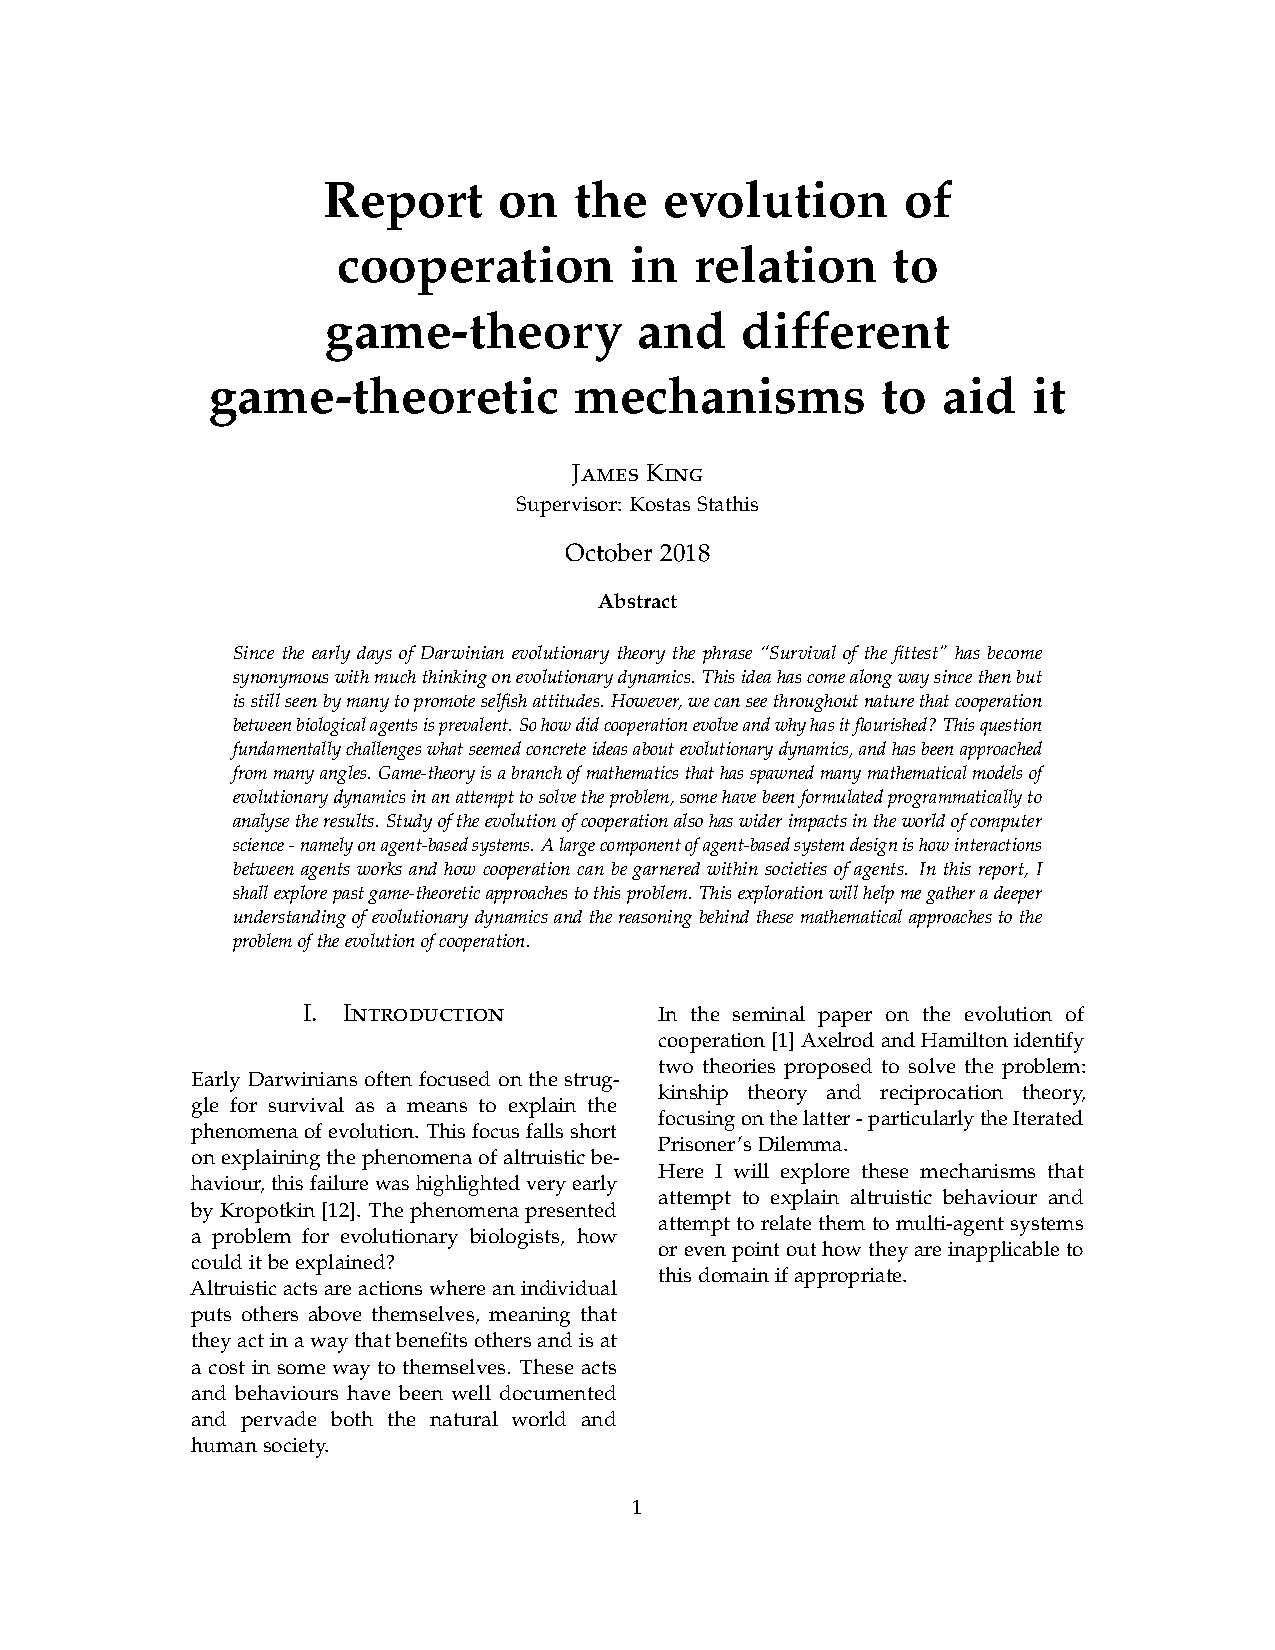
\includepdf[pages=-]{../../EvolCoop/EvolCoopReport.pdf}

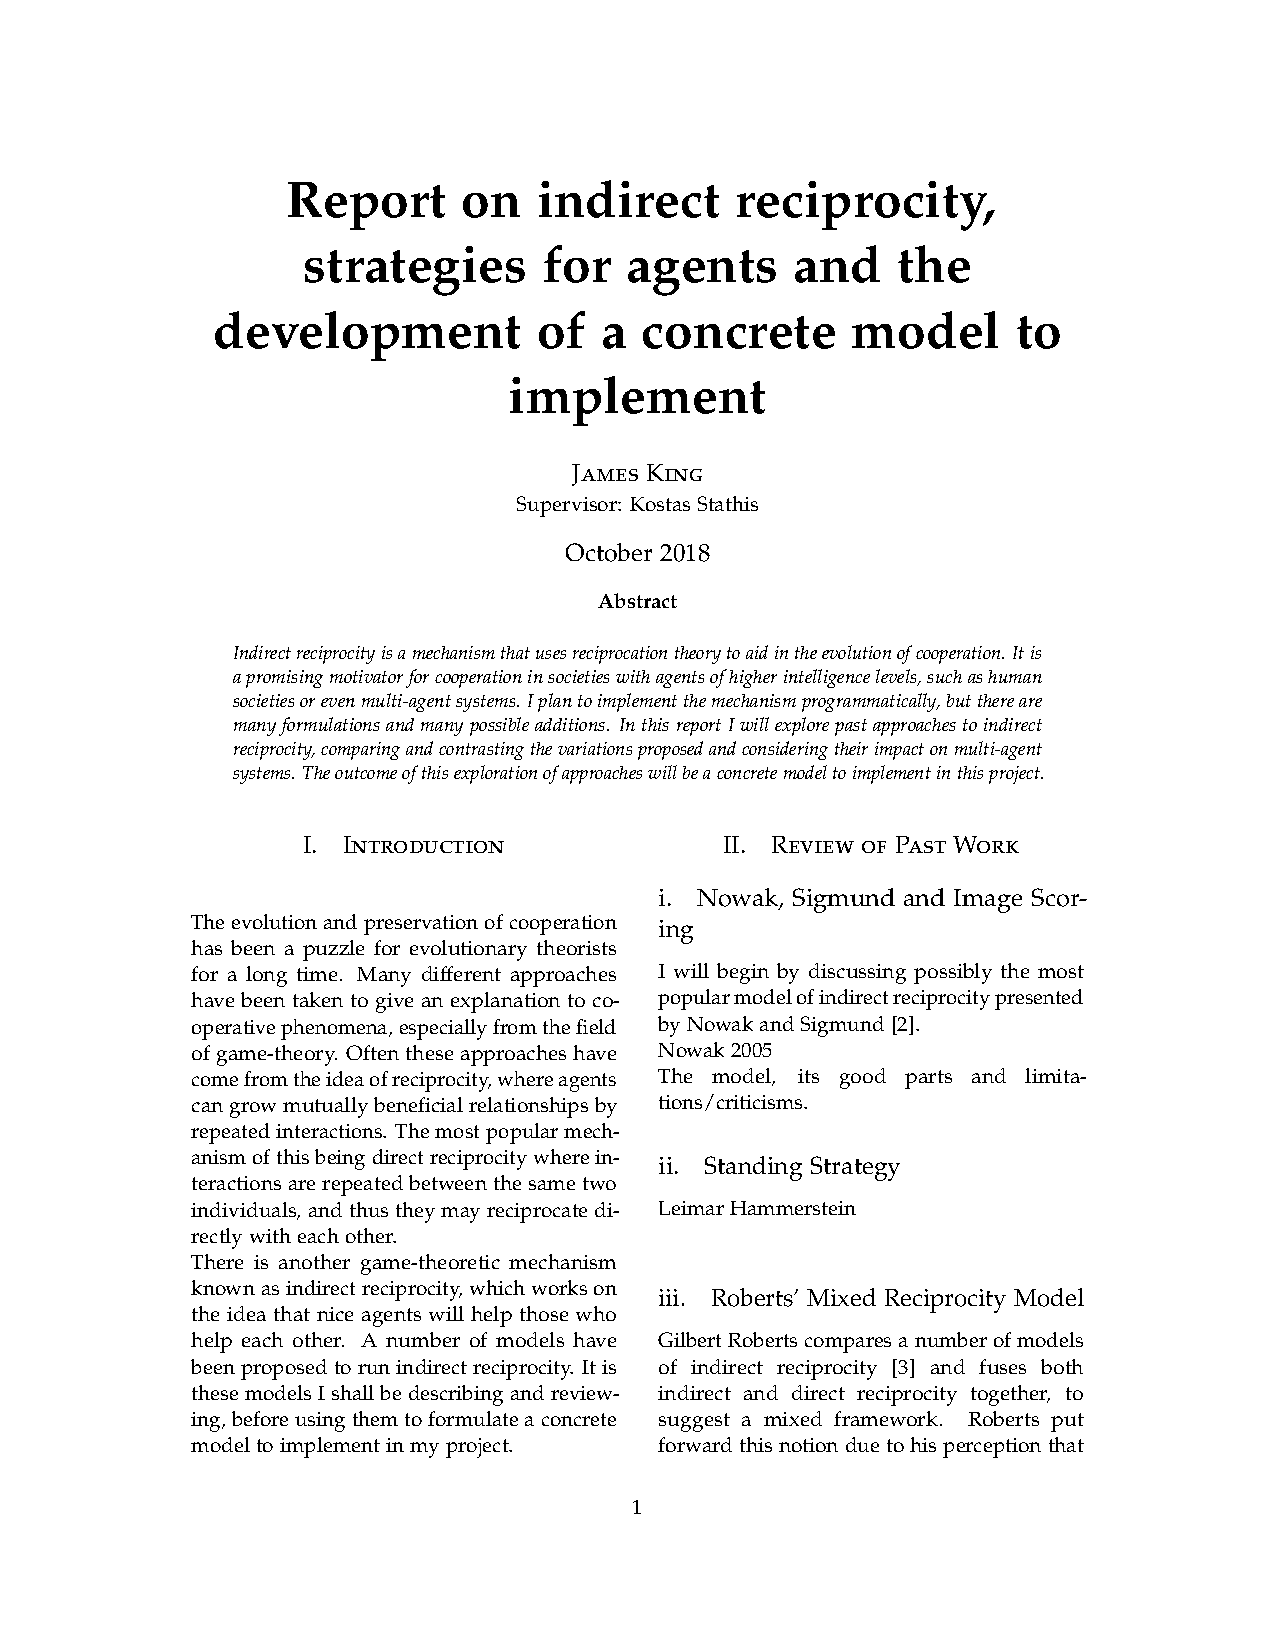
\includepdf[pages=-]{../../IndirRec/IndirRec.pdf}

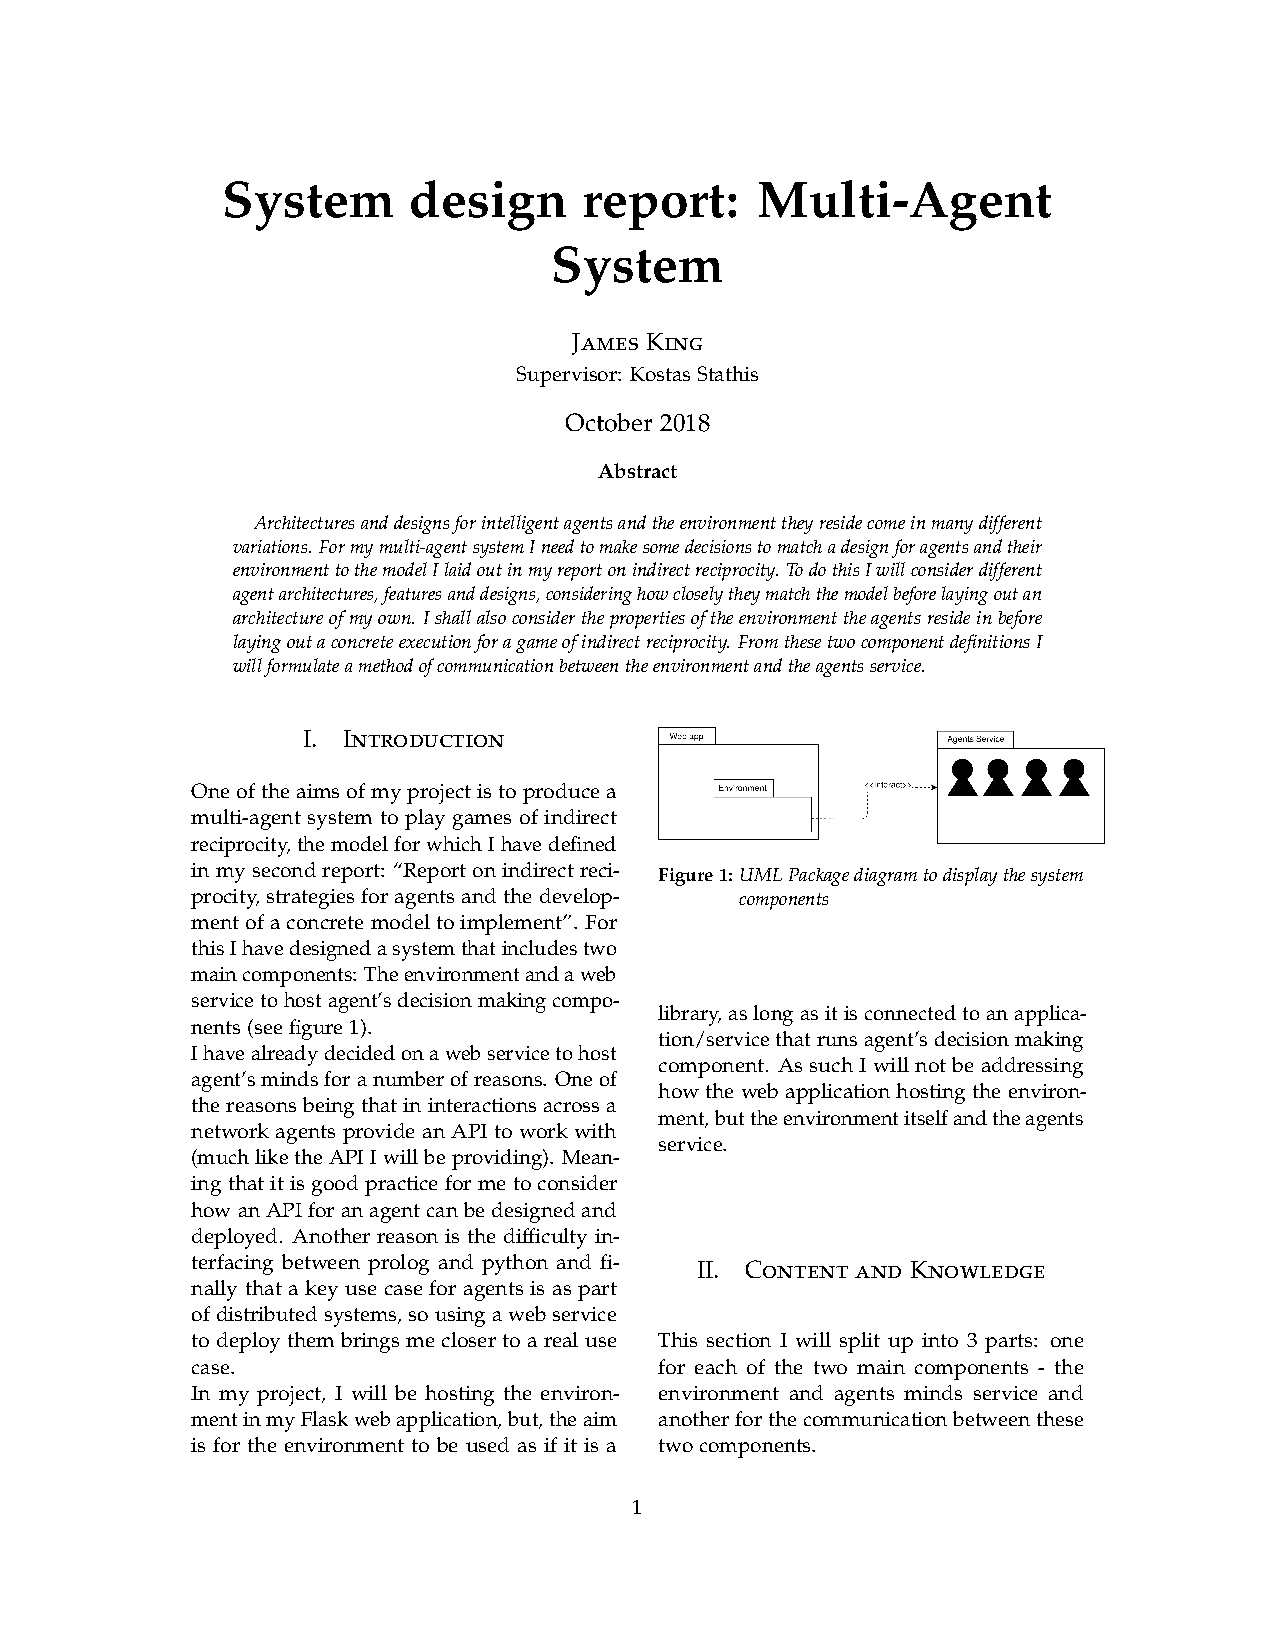
\includepdf[pages=-]{../../SysDesign/SysDesign.pdf}

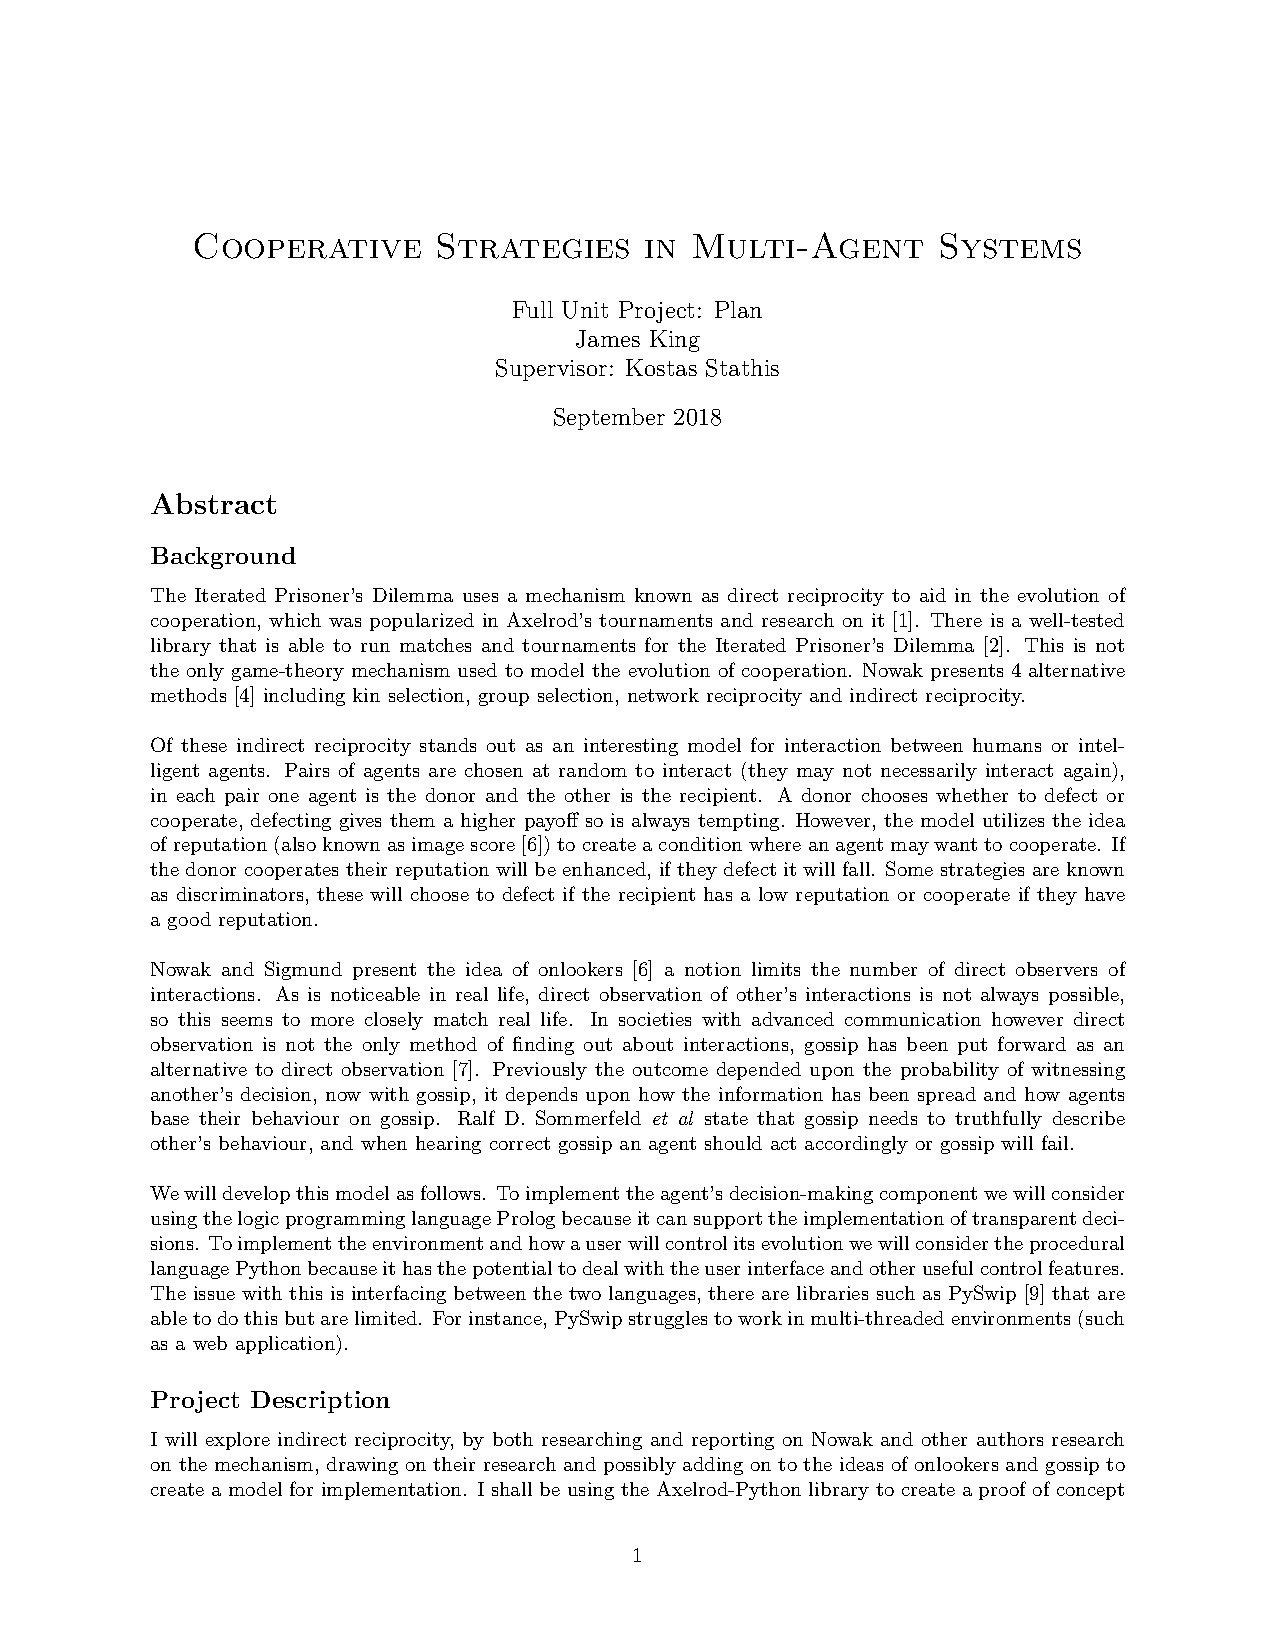
\includepdf[pages=-]{../../2ProjectPlan/ProjectPlan2.pdf}

\end{document}

\end{article}
